\chapter{Implementation}
\label{ch: Chapter3}

\section{Agent and Web Server Communication}

% Talk about Zero MQ
All three agents communicate with each other and the web server using the Zero
MQ asynchronous messaging library. Essentially, this library
works as a way to implement inter process communication without a message
broker~\cite{zeromq}. In other words, different processes are able to communicate with each
other without any central bus. This is convenient as fewer processes are needed
for the system to function. Lowering the number of overall processes lowers the
RAM and CPU usage of the software. The library is ported to many different
programming languages; however we are using the Python port titled Pyzmq to
implement in our code base.
%
\begin{figure}
    \centering
    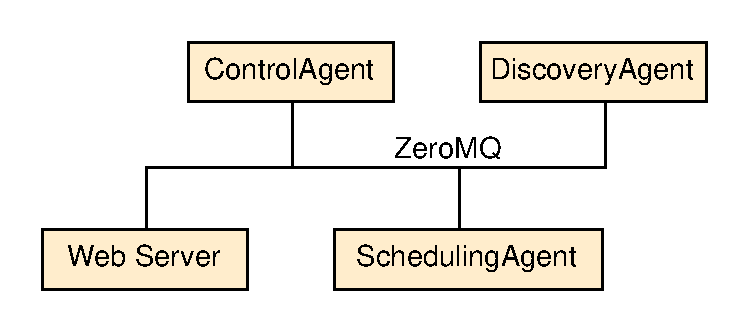
\includegraphics[width=0.4\textwidth]{figs/pubSubAgents.pdf}
    \caption{Publish Subscribe Communication using ZeroMQ}
    \label{fig:pubSubAgents}
\end{figure}

More specifically, the publish subscribe model of communication is used where
each agent communicates via a socket where each socket responds to a specific
topic. The topics and port numbers are listed below along with their
corresponding agents in Table~\ref{tab:pubsubspecs}. %
%
\begin{table}
    \centering
    \begin{tabular}{|c|c|c|}
        \hline
        Agent & Topic & Port Number\\
        \hline
        Discovery Agent & "discovery" & 5556\\
        Scheduling Agent & "scheduling" & 5556\\
        Control Agent & "control" & 5556\\
        \hline
    \end{tabular}
    \caption{Publish/Subscribe Communication Specifications}
    \label{tab:pubsubspecs}
\end{table}
%
In order to send data between the different processes, the topic, method, and
data are delimited in a particular way. This method is shown below as follows: %
%
\begin{verbatim}
    topic method/args
\end{verbatim}
%
A space cannot be included between the method name and arguments as this
interferes with the Python \texttt{split} method for extracting the fields. The
\texttt{topic} is the string described previously, the \texttt{method} is the
name of the desired method to be called on the agent object, and \texttt{args}
is the arguments supplied to the desired method. In order to send a message to
an agent, the \texttt{publish} method defined in the \texttt{pubsub} module
should be called. An optional argument titled \texttt{cycleCount} is available
which will allow the publish message to be sent multiple times. During testing,
it was found that during the transmission of some messages, this was necessary
due to the way ZeroMQ is implemented.

\section{Agent Functionality}
The agents contained in the software are associated with a Python class of the
same name. Each class is instantiated and run with specifications declared in
Table~\ref{tab:pubsubspecs}. Some of the methods defined in each class will be
described in the following subsections.

\subsection{Control Agent Functionality}
The flow chart of method \texttt{setDeviceStatus} is shown in
Figure~\ref{fig:setDeviceStatus}. The purpose of this method is to set the
status of the desired device. When the method is called, the data dictionary is
obtained which contains the device ID. With this device ID, the API type can be
determined using the SQLite database. Subsequently, the appropriate device API
module can be imported. If the power state exists as a key in the device data
dictionary, the power state of the WeMo Insight Switch will be set as ON or OFF.
If the duty cycle key exists, the duty cycle of the single board computer motor
drivers is set. If the shutdown key is set, the single board computer is
shutdown. In order to reconnect to the single board computer, the board must be
started and receiver program ran. If necessary, the device must be reconnected
to the WiFi network. %
%
\begin{figure}
    \centering
    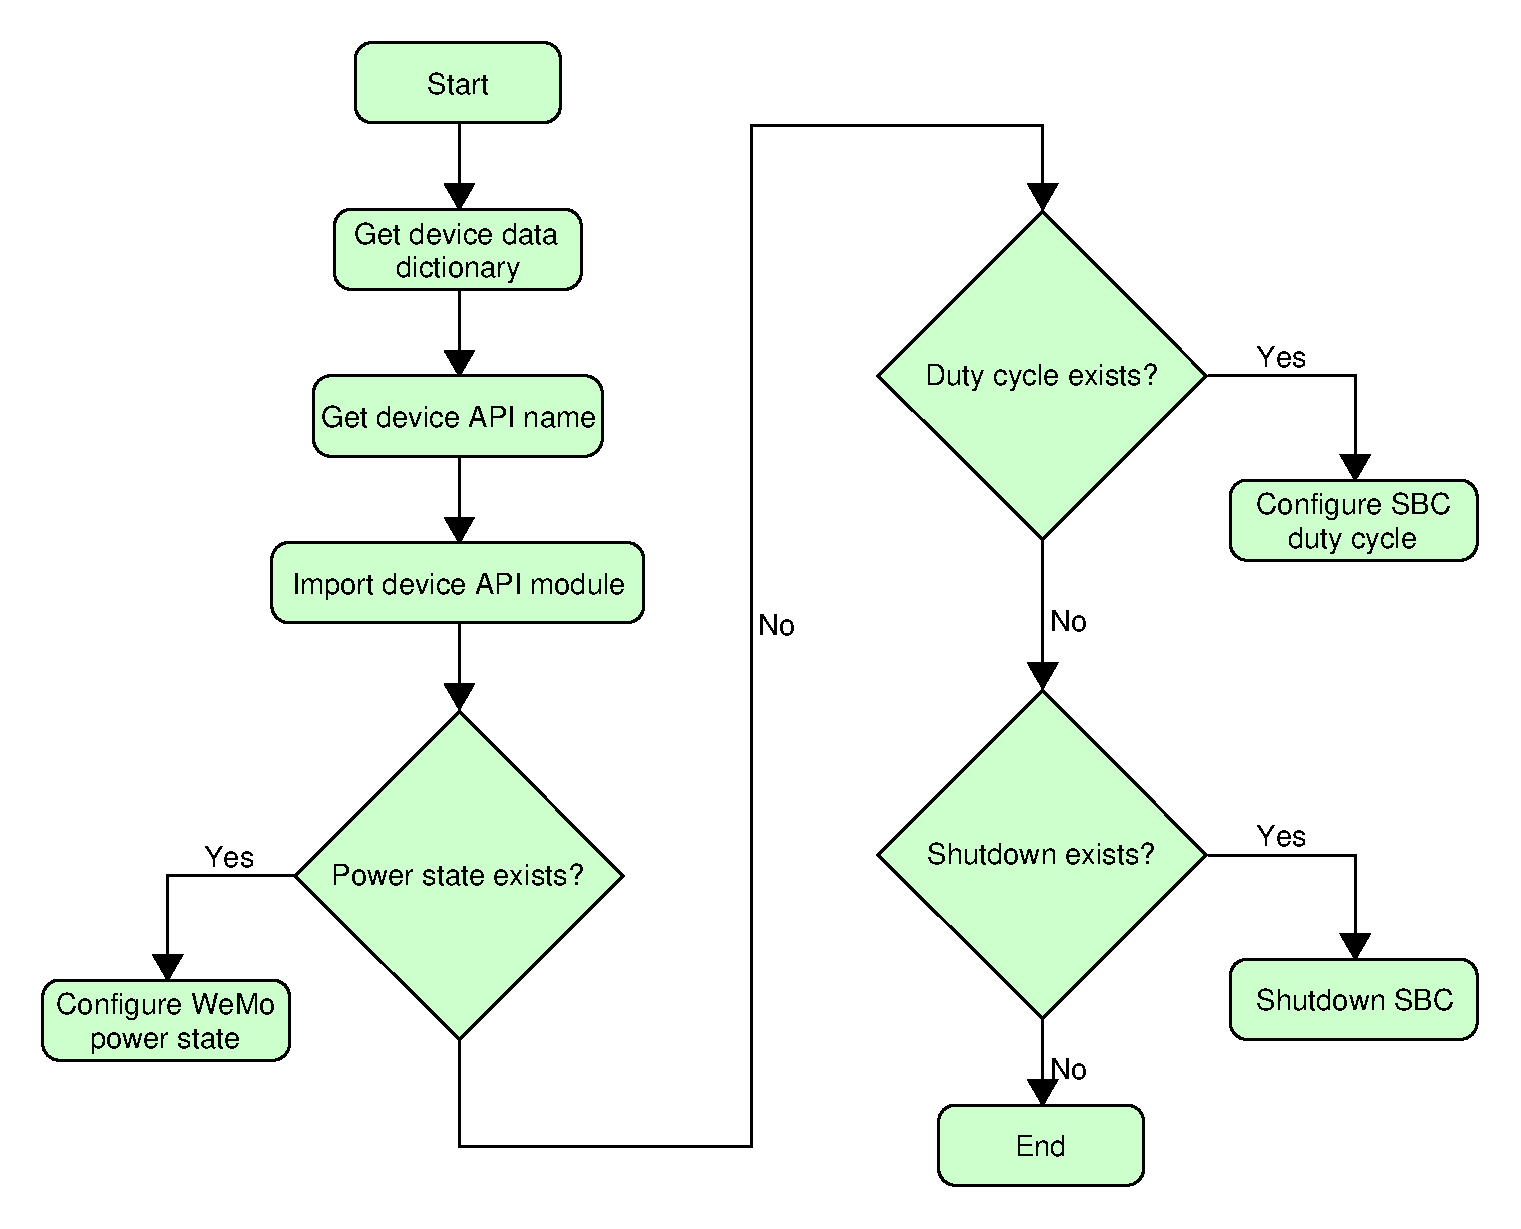
\includegraphics[scale=0.5]{figs/setDeviceStatus.pdf}
    \caption{setDeviceStatus Flow Chart}
    \label{fig:setDeviceStatus}
\end{figure}

To obtain necessary data quantities from the device, the
\texttt{getDeviceStatus} method, defined in Figure~\ref{fig:getDeviceStatus}, is called. Once the proper data parameters are
obtained, the \texttt{getState} function defined in the devices API module can
be called with the data parameters such as power state and
status. Once the agent has finished sending these to the device, a request is
sent to the web server to inform the server that it completed searching for the
required device data. %

%
\begin{figure}
    \centering
    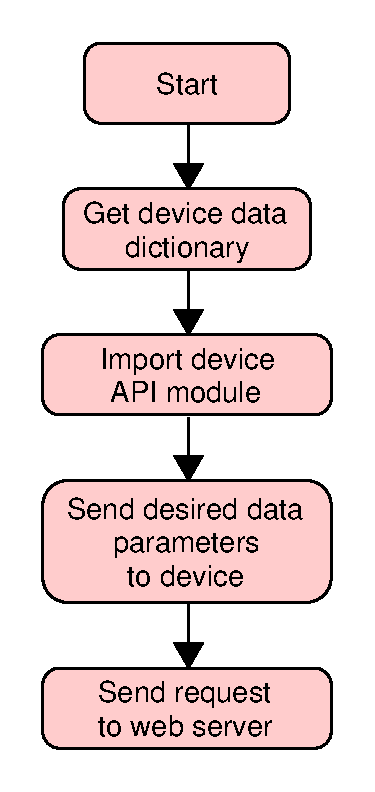
\includegraphics[scale=0.5]{figs/getDeviceStatus.pdf}
    \caption{getDeviceStatus Flow Chart}
    \label{fig:getDeviceStatus}
\end{figure}

Every device connected to iBEMS will have a thread associated with it started from the control agent. This thread will run the \texttt{periodicQueryBehavior} method to periodically query for device data and store in the corresponding Cassandra database table. A user specified delay is placed in the class's module to prevent the thread from overwhelming the system.
\begin{figure}[H]
    \centering
    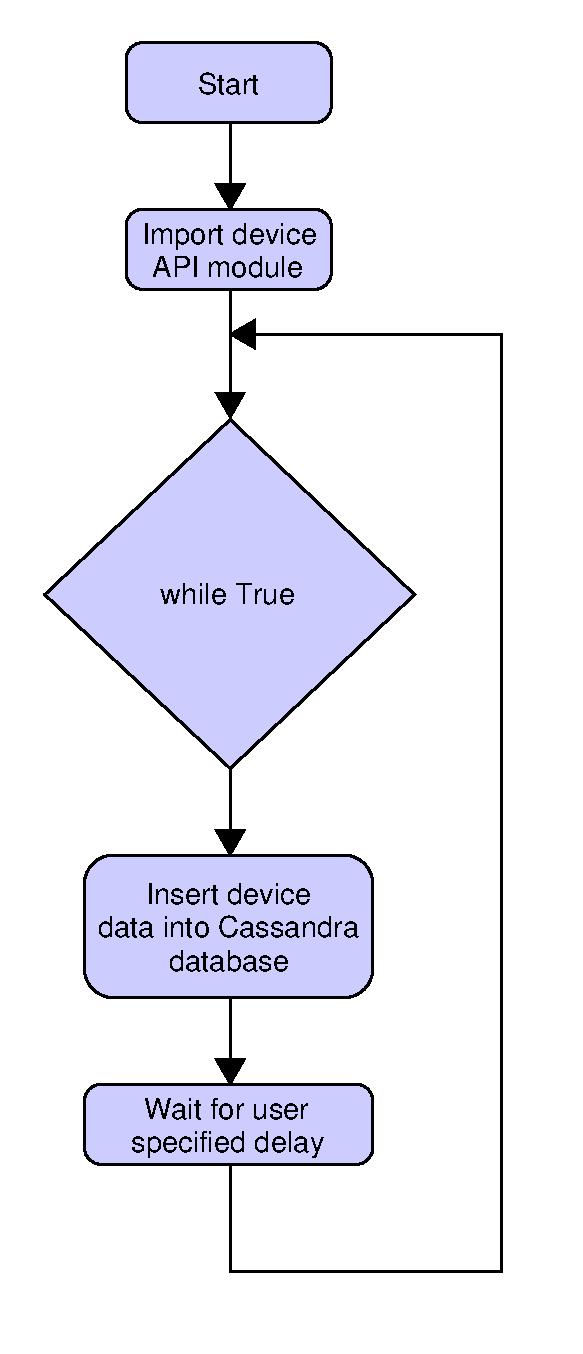
\includegraphics[scale=0.5]{figs/periodicQueryBehavior.pdf}
    \caption{periodicQueryBehavior Flow Chart}
    \label{fig:periodicQueryBehavior}
\end{figure}
To reduce latency, the device status is retrieved directly from the API module in the \texttt{periodicQueryBehavior} method rather than calling \texttt{getDeviceStatus} as this prevents the API from being imported unnecessarily.

\subsection{Discovery Agent Functionality}
The purpose of the discovery agent is to search for devices that respond to the supported APIs by the software. A flow chart demonstrating the \texttt{searchForDevices} method is shown in Figure~\ref{fig:searchForDevices}. This method is called whenever the active devices page is loaded. The algorithm could be improved to help page load times. All the device APIs are loaded in the \texttt{findDevices} function defined in each device's API module is called which will return a list of found URLs. Once the device's URL is determined, it's metadata can be passed to the \texttt{setDeviceToActive} method which will set up the device in the two databases.

\begin{figure}[H]
    \centering
    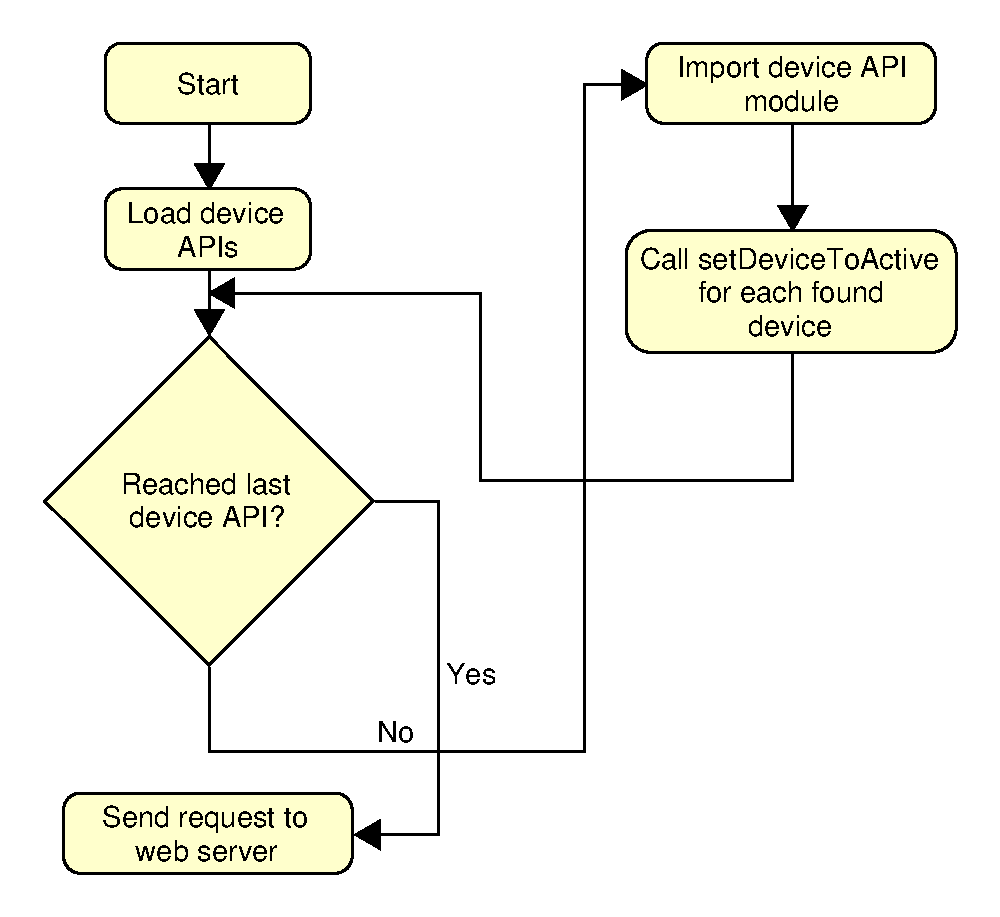
\includegraphics[scale=0.5]{figs/searchForDevices.pdf}
    \caption{searchForDevices Flow Chart}
    \label{fig:searchForDevices}
\end{figure}
The \texttt{setDeviceToActive} shown in Figure~\ref{fig:setDeviceToActive} will first check to make sure the device is not already in the active devices table. Then, it will add the device to the active devices table, create a table in the Cassandra database for storing time-series data, send a message to the scheduling agent to check for schedule updates, and send a message to the control agent to start collecting data.
\begin{figure}[H]
    \centering
    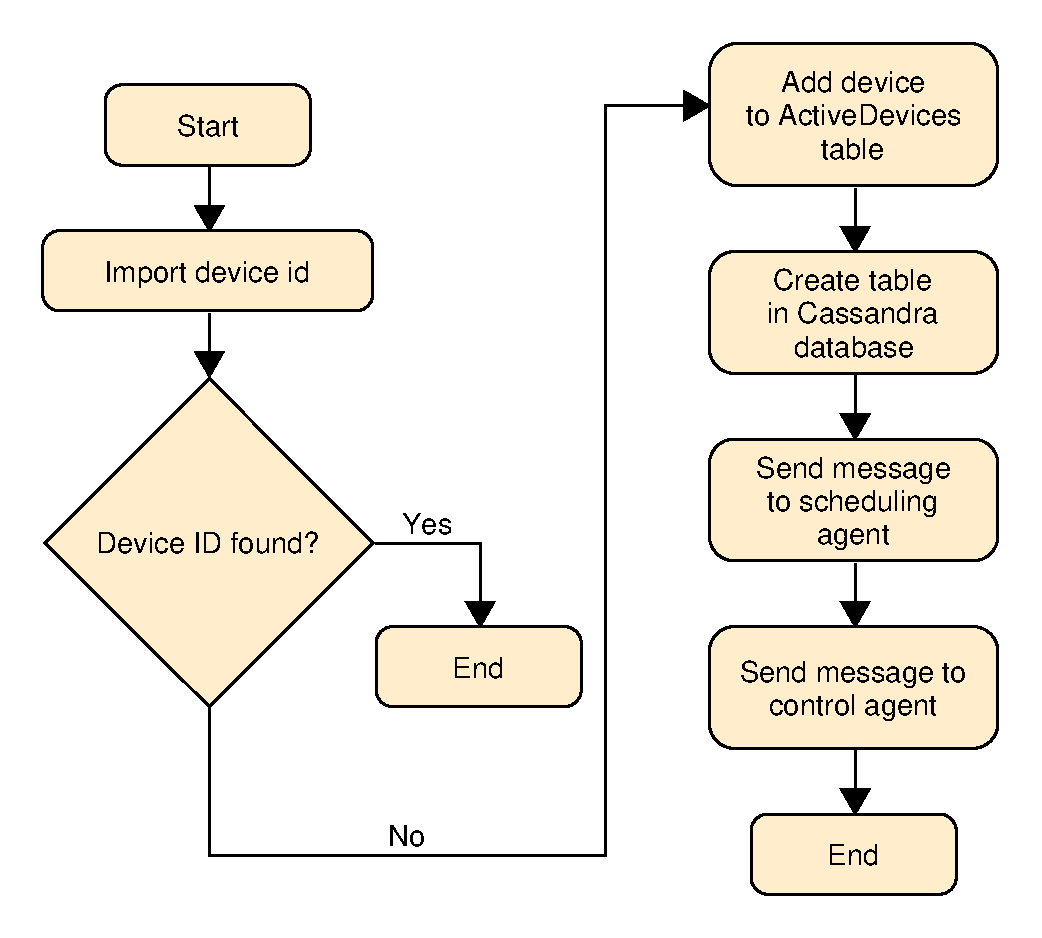
\includegraphics[scale=0.5]{figs/setDeviceToActive.pdf}
    \caption{setDeviceToActive Flow Chart}
    \label{fig:setDeviceToActive}
\end{figure}

\subsection{Scheduling Agent Functionality}
The scheduling agent is able to update the device status of each device dependent on whether a schedule is set for the specific time period and day. One of the methods that is called, \texttt{updateScheduleFromServer} is invoked when the user presses the \say{Update Schedule} button from the UI on the scheduling page. A flow chart of this method is shown in Figure~\ref{fig:updateScheduleFromServer}. When this method is called the desired schedule is loaded in as a dictionary and parsed to extract the necessary periods and given day. First the times are stored in military time in the database for more convenient storage and parsing later on. Then, a table is created in the Apache Cassandra database for the device for the provided data and the device ID is embedded. The table's data is destroyed to ensure there are no errors regarding overlapping schedules. Lastly, all the scheduling periods extracted from the dictionary are stored as rows in the table. 
\begin{figure}[H]
    \centering
    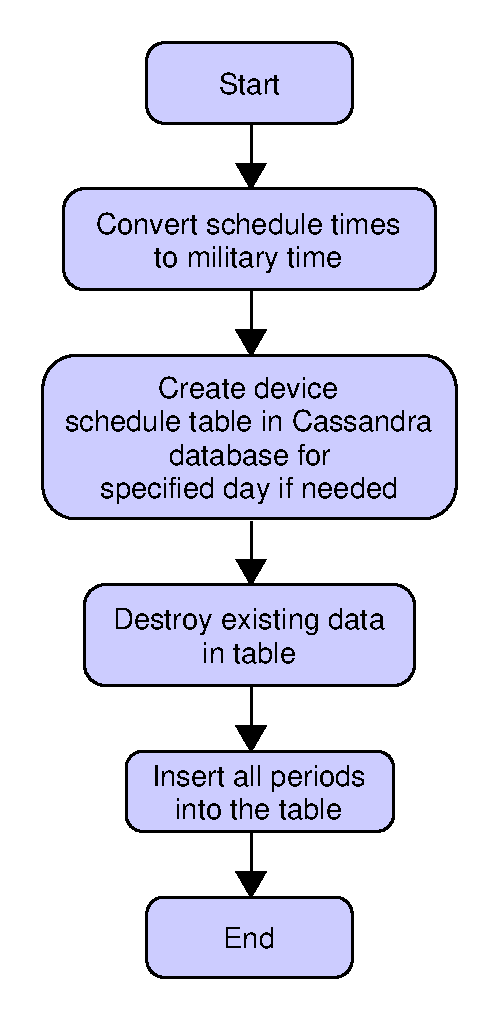
\includegraphics[scale=0.5]{figs/updateScheduleFromServer.pdf}
    \caption{updateScheduleFromServer Flow Chart}
    \label{fig:updateScheduleFromServer}
\end{figure}
A second method that is run inside each device thread is \texttt{periodicDeviceUpdateMethod}, defined in Figure~\ref{fig:periodicDeviceUpdateMethod}, is started when the discovery agent sets the discovered device to active. By first loading the device's API name, the scheduling agent can begin checking for scheduling periods inside an infinite loop. The status dictionary is queried from the Cassandra database and loaded into a dictionary. All these scheduling periods are looped over for the current day while constantly checking whether the current time in seconds is within the starting and ending time. A conversion of both starting and ending time to seconds is necessary as it is challenging to work with these quantities in standard and military time when comparing times. If the current time does lie inside the scheduling period, the device's state is set dependent on the API. 
\begin{figure}[H]
    \centering
    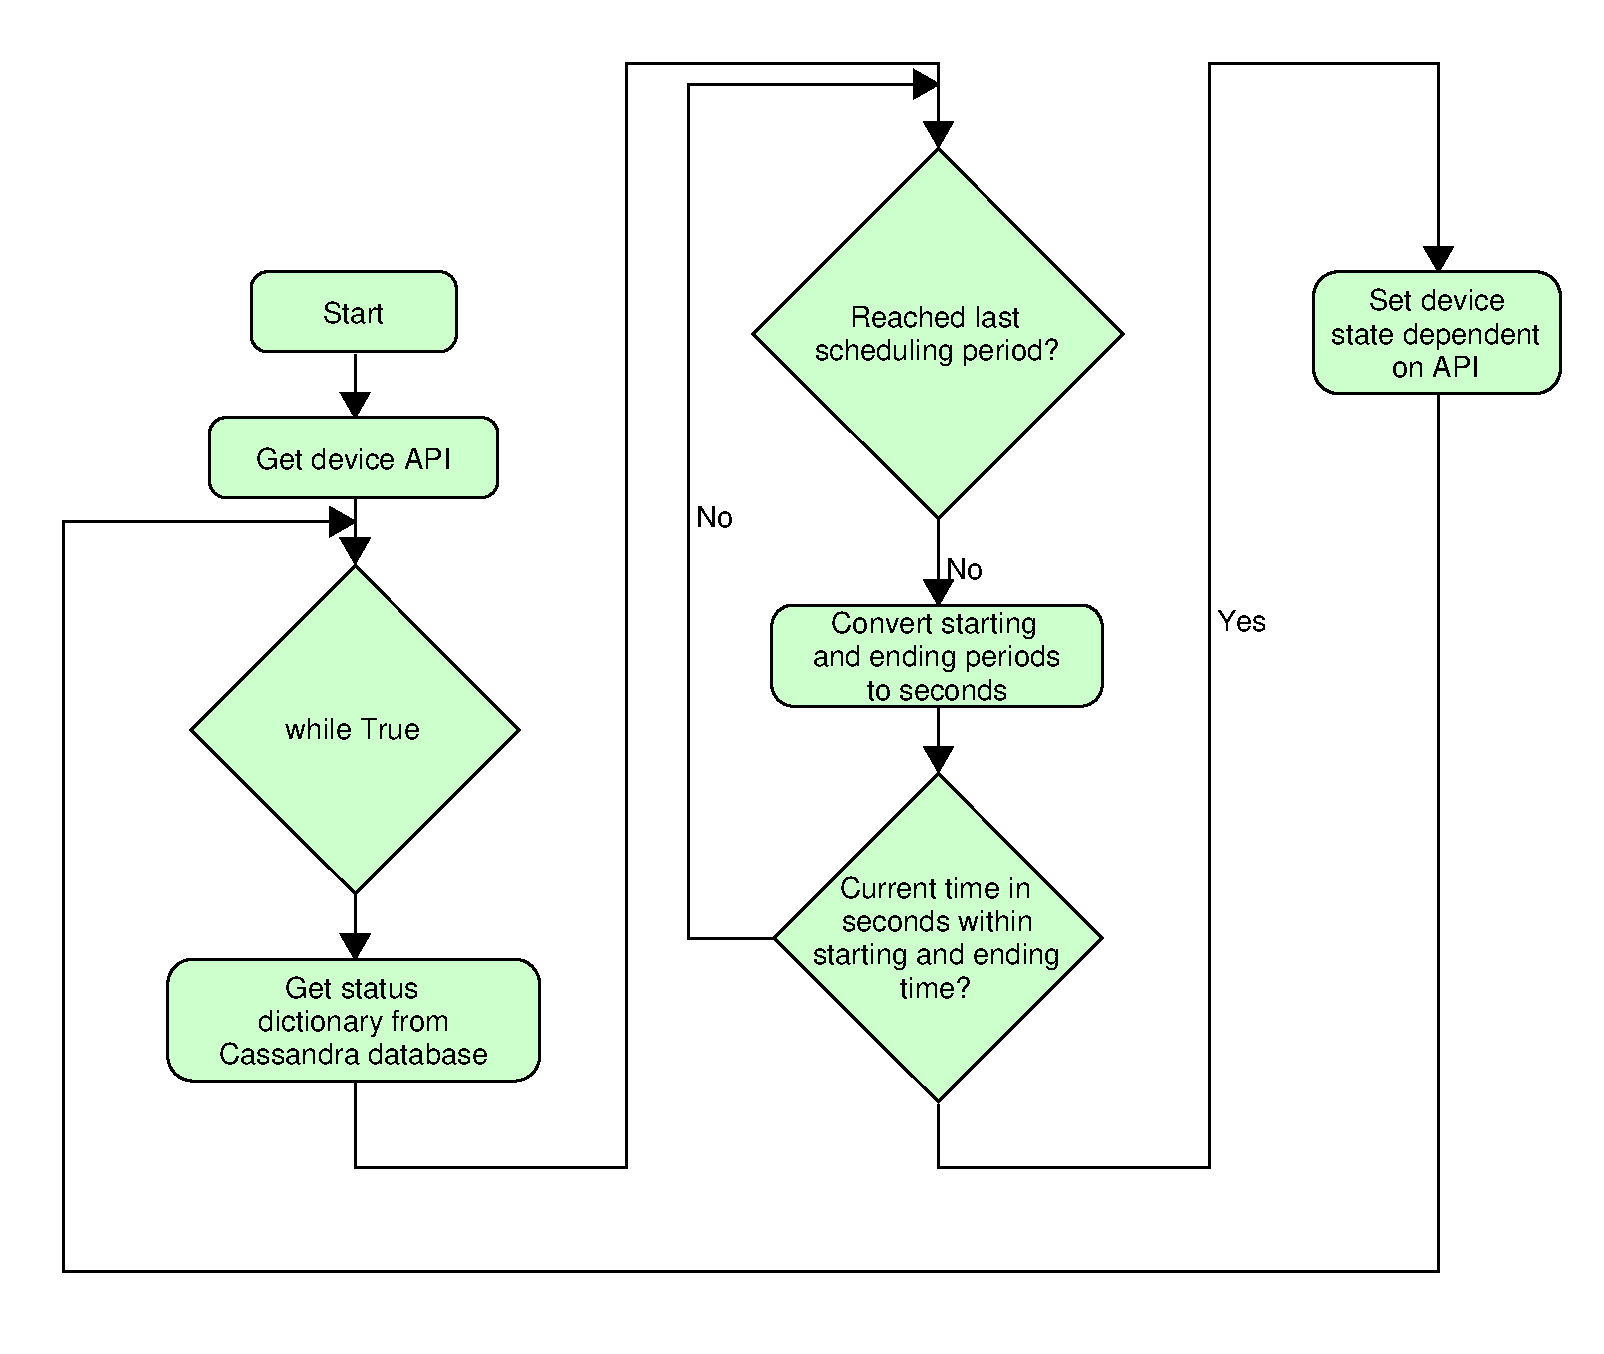
\includegraphics[scale=0.5]{figs/periodicDeviceUpdateMethod.pdf}
    \caption{periodicDeviceUpdateMethod Flow Chart}
    \label{fig:periodicDeviceUpdateMethod}
\end{figure}

\section{Desktop GUI Functionality}
The functionality of the desktop GUI launched when the user runs the Python script titled \texttt{GUI.py} is shown in Figure~\ref{fig:desktopgui}. Packages used to construct the GUI include tkinter which is a Python interface for the Tcl/Tk GUI toolkit. When the GUI is started up, the title, buttons, and labels are created along with ties to the callback functions \texttt{startCallback} and \texttt{stopCallback}. The \texttt{startCallback} function is called when the user presses the \say{Start iBEMS} button. This function first checks whether iBEMS is already running by checking for processes already running on the machine including the web server itself and the three agents. This is performed using the command \texttt{ps -aux}. After this has been completed, an error popup is shown preventing another instance of the software from running. This prevents errors associated with copies of agents and web servers running simultaneously. To properly stop the software, the \say{Stop iBEMS} button will shutdown the software by first finding the process ID's associated with the agents and web server. To perform this, it will place the output of \texttt{ps -aux | grep [process]} into a text file where \say{process} is the name of the target process. A file descriptor of the process status output text file is instantiated and all the lines are read in to be parsed. Each process output is split by spaces and the second element in the list is denoted as the process id. Then, using the \texttt{kill} command, these processes are killed. 
\begin{figure}[H]
    \centering
    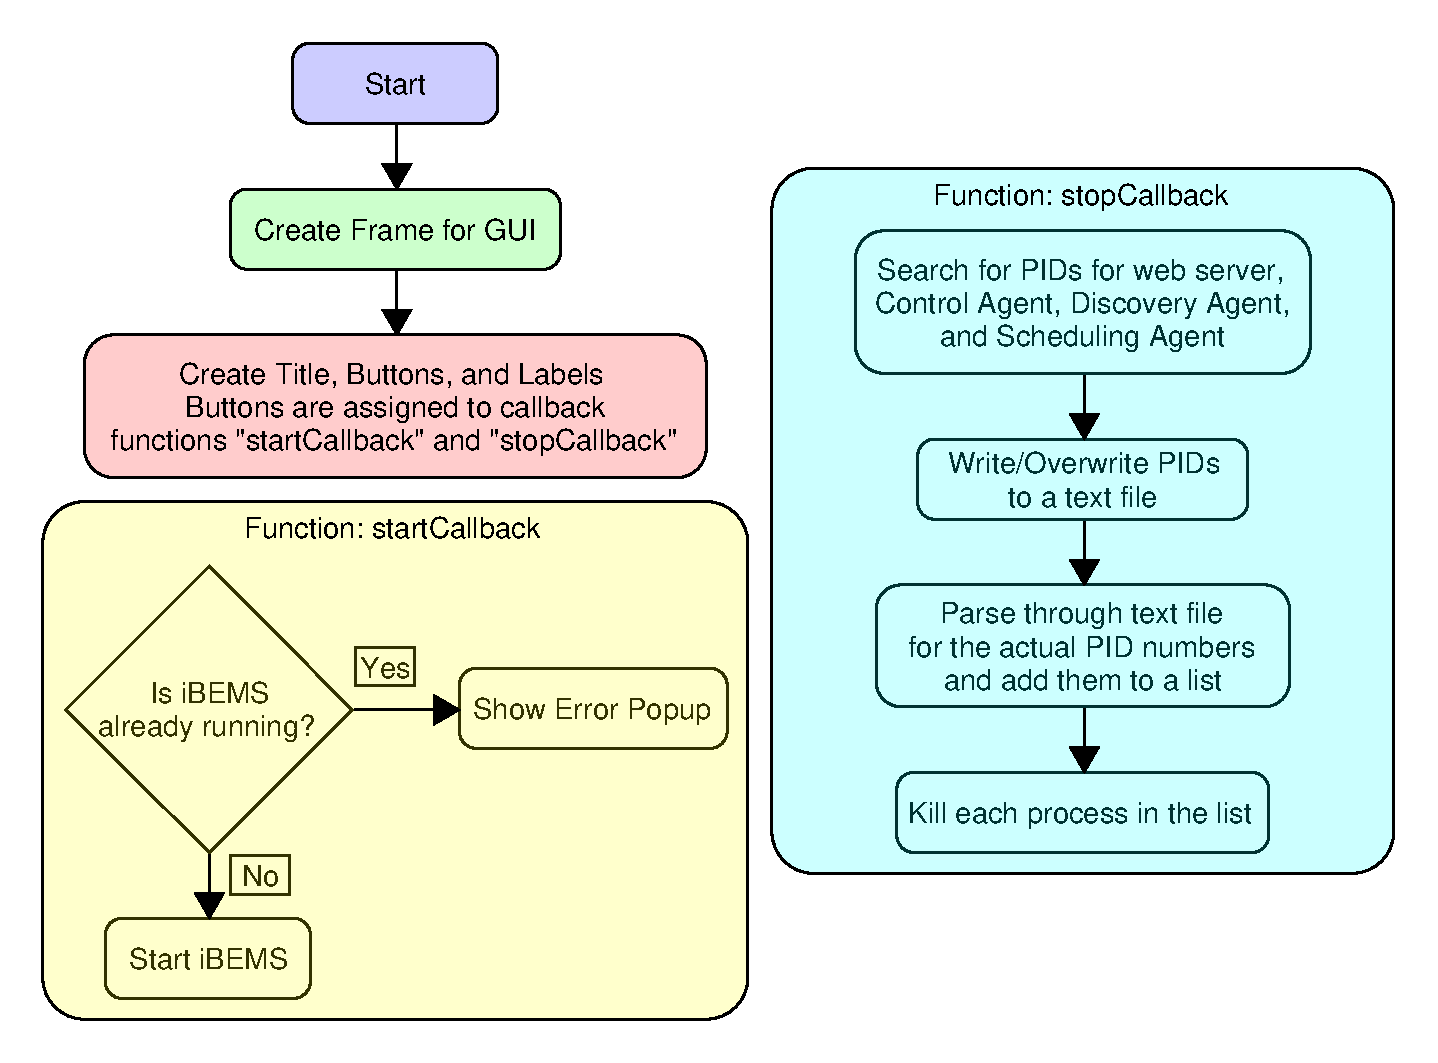
\includegraphics[scale=0.6]{figs/GUI_Diagram.pdf}
    \caption{Python desktop GUI Functionality}
    \label{fig:desktopgui}
\end{figure}

\section{Embedded Computer}

\begin{figure}[H]
    \centering
    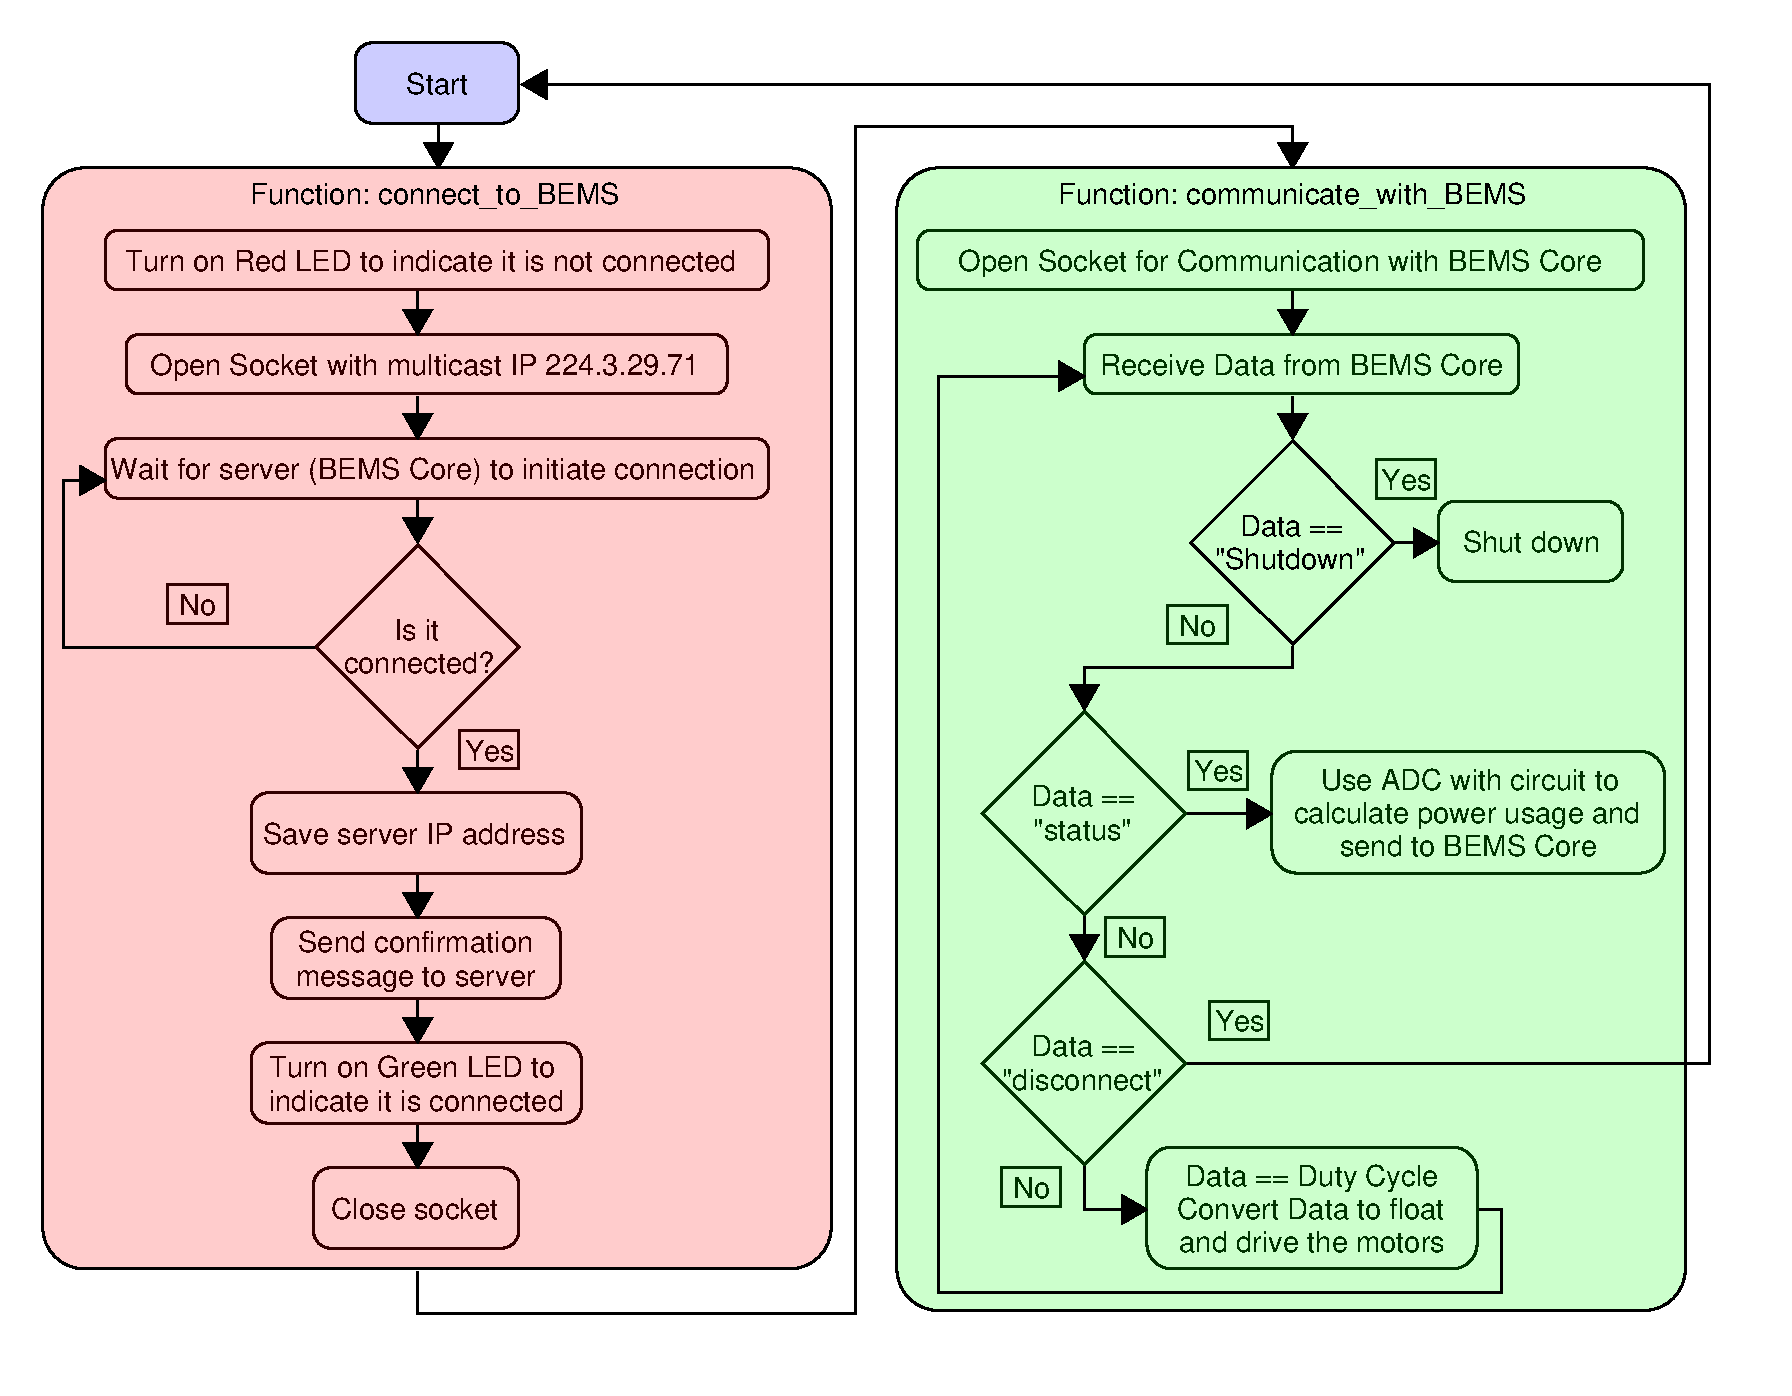
\includegraphics[scale=0.5]{figs/Beaglebone_Receiver_Diagram.pdf}
    \caption{Receiver Running on Embedded Computer}
    \label{fig:Beaglebone_Receiver_Diagram}
\end{figure}

The embedded computer needed some software to be able to connect to and communicate with the iBEMS Core. To achieve this, a program consisting of 2 functions for connecting and communicating is used.
\medbreak
The first of these functions is \texttt{connect\_to\_iBEMS}. This function first turns on the red LED on the embedded computer to indicate it is not yet connected. Then it creates a socket using a multicast IP address that the corresponding API in the iBEMS core will be looking for. Once the socket is created, the embedded computer will enter a loop and wait for the iBEMS core to make the initial connection. When that connection is made, it will exit the loop, save the IP address of the iBEMS core, send a confirmation message, then turn on the green LED before closing the multicast socket.
\medbreak
The second function, \texttt{communicate\_with\_iBEMS} will open another socket but with the IP address of the iBEMS core found in \texttt{connect\_to\_iBEMS}. It will then enter a indefinite loop to continually receive data from the iBEMS core. There are 4 different messages that the iBEMS core sends to the embedded computer. First, it will check if the iBEMS core is telling it to shut down with the command \say{Shutdown}. If so, the embedded computer will immediately shut down. Second, if the data sent by iBEMS is \say{status}, the embedded computer will take a reading from the circuit described in Chapter~\ref{ch: Chapter2} section 3. In case the user decides to shut down the iBEMS core without turning off the embedded computer, another message \say{disconnect} will be sent in which case the embedded computer will exit \texttt{communicate\_with\_iBEMS} and start the entire program over again. Finally, if iBEMS is not sending any of the above options, it means that the user is sending a new duty cycle to drive the motors with. Since iBEMS only sends messages with the string data type, this has to be converted to a float in order to call the motor driver function. 


%%% Local Variables:
%%% mode: latex
%%% TeX-master: "../finalReport"
%%% End:
